\chapter{Неймовірна радість моделювання} 
\label{chap:first}

Останнім серйозним завданням у даній лабораторній роботі було моделювання цього всього добра на ПК. Оскільки автор належить до тих божевільних, які у неземному захваті від операційних систем на базі ядра Linux, було прийняте надзвичайно складне рішення: обрати стареньку, але все ще здатну дати прочуханки новішим недопрограмам, написаним мавпочками, програму Qucs. Інтерфейс програми надзвичайно простий, а взаємодія із користувачем шедевральна. Її вигляд зоображений на рис. \ref{fig:qucs}.

\begin{figure}[h]
\center{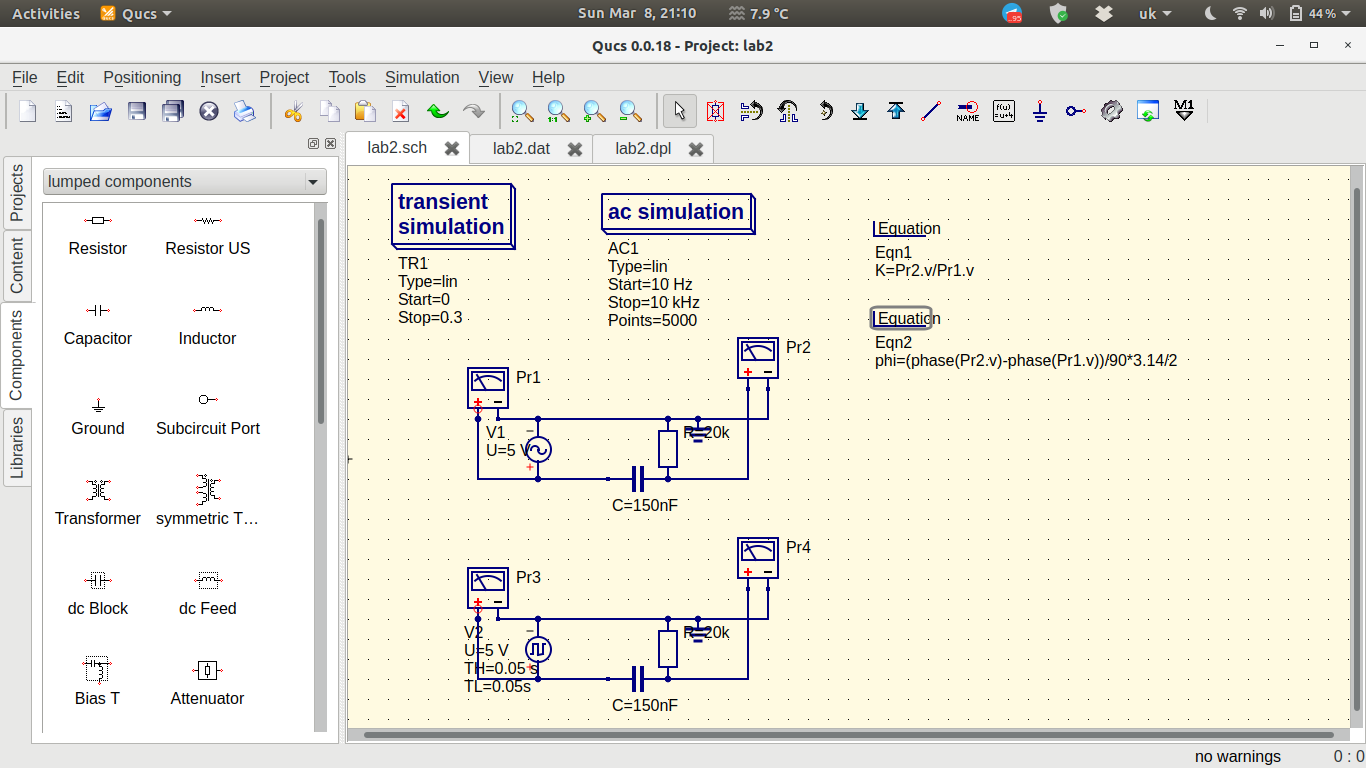
\includegraphics[width=1\linewidth]{modelling/window.png}}
\caption{Робота в програмі Qucs. Зображено моделювання диферинціюючого чотирьохполюсника.}
\label{fig:qucs}
\end{figure}

Отримані результати роботи в цій програмі дали змогу знайти декілька суттєвих помилок у експериментальній частині, що ще раз підкреслює важливість моделювання. На рисунках \ref{fig:modkph} зображені графіки АЧХ та ФЧХ, а також осцилограма для різних чотирьохполюсників.

\begin{figure}[h]
    \begin{minipage}[h]{0.47\linewidth}
        \center{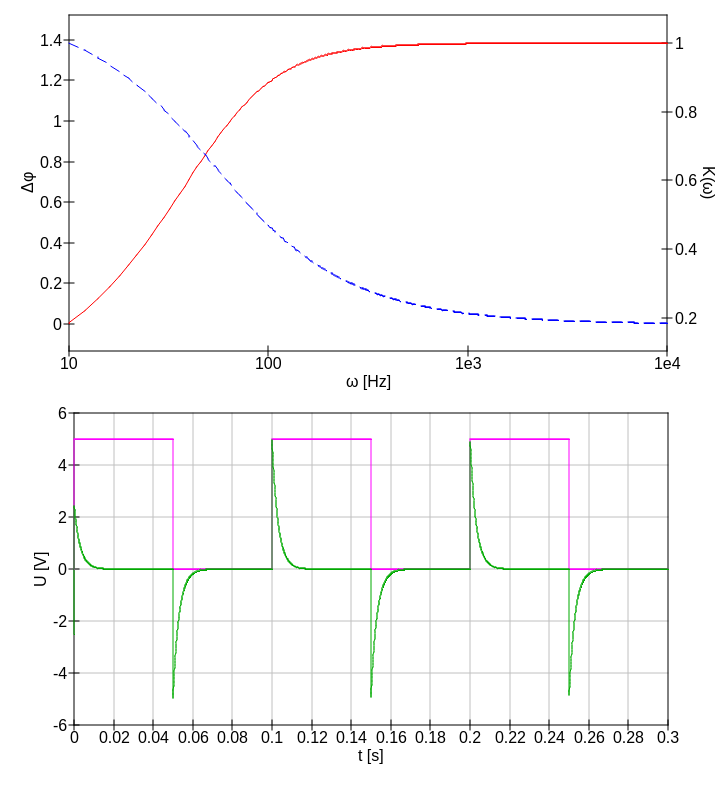
\includegraphics[width=1\linewidth]{modelling/dif_KPHI.png}} \\Диферинціювальний
    \end{minipage}
    \hfill
    \begin{minipage}[h]{0.47\linewidth}
        \center{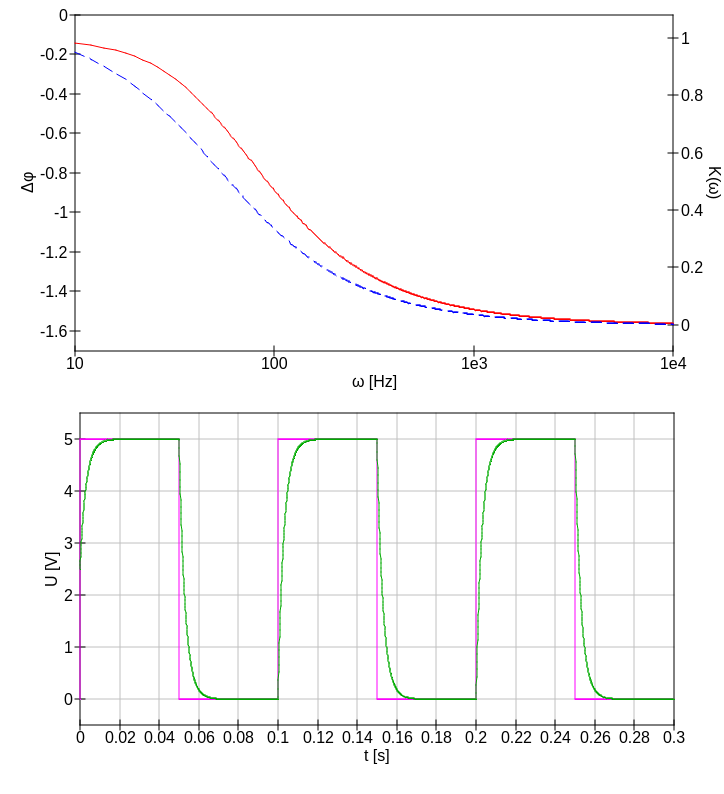
\includegraphics[width=1\linewidth]{modelling/KPHI.png}} \\Інтегрувальний
    \end{minipage}
    \caption{Отримані теоретичні залежності відношення амплітуд $K(\omega)$ (червона, суцільна) та зсуву фаз $\phi(\omega)$ (синя, пунктир) при $R = 20k\Omega$ та $C = 150nF$ (зверху). Осцилограма для квардратного вхідного імпульсу, із заповненням $50\%$ напругою $U=5V$ та частотою $\omega = 10Hz$ (знизу).}
    \label{fig:modkph}
\end{figure}